\section{Signal/background comparisons}
\label{app:SignalBackgroundComparison}

\subsection{BDT input variables}
\label{subapp:SOVERB_BDTInputVars}
Figures \ref{fig:SOVERB_BDTInputs_Hp} compare the shape of the variables included in the BDT for all $H^{+}$ signal masses and background in the SR.

\begin{figure}[H]
    \subfloat[HT\_jets] {
        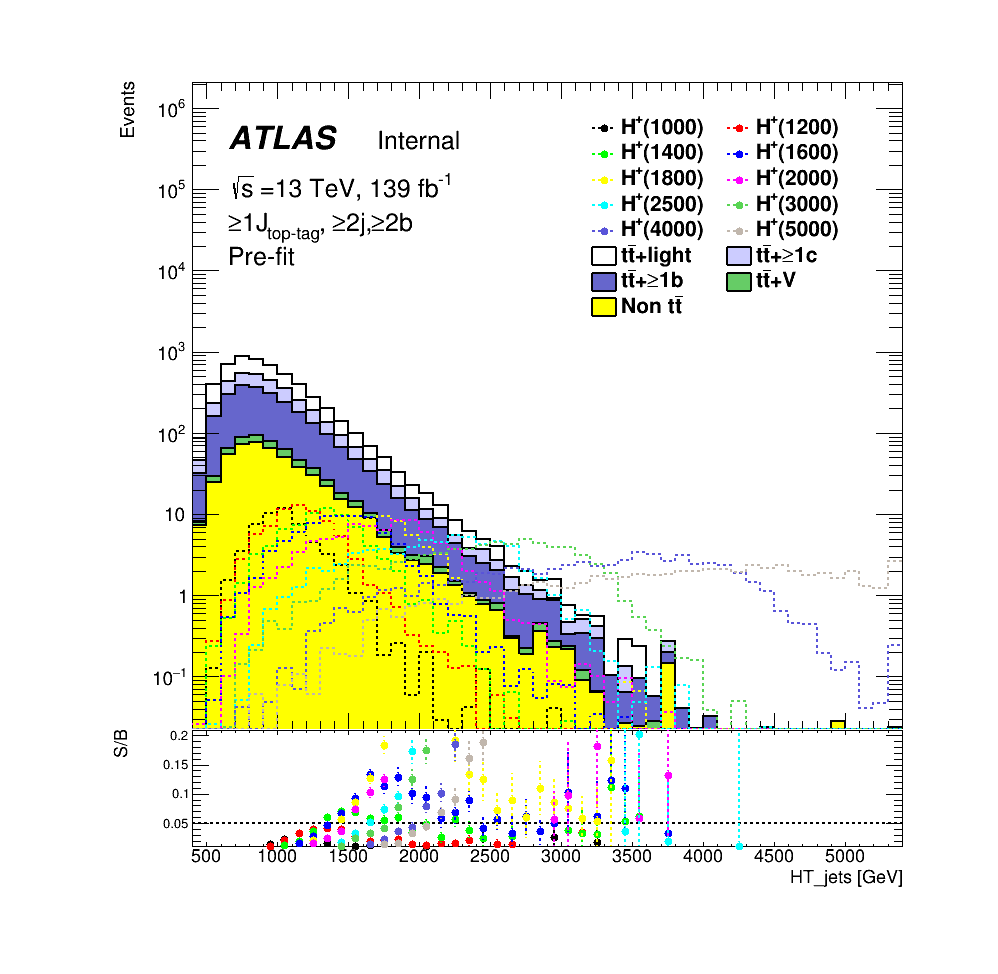
\includegraphics[width=0.50\textwidth]{images/SigBkgComparison/SOVERB_HTjets_beforeRW_geq1tgeq2jgeq2b.png}
        \label{fig:SOVERB_HT_jets}
    }
    \subfloat[LeadingJet\_pt] {
        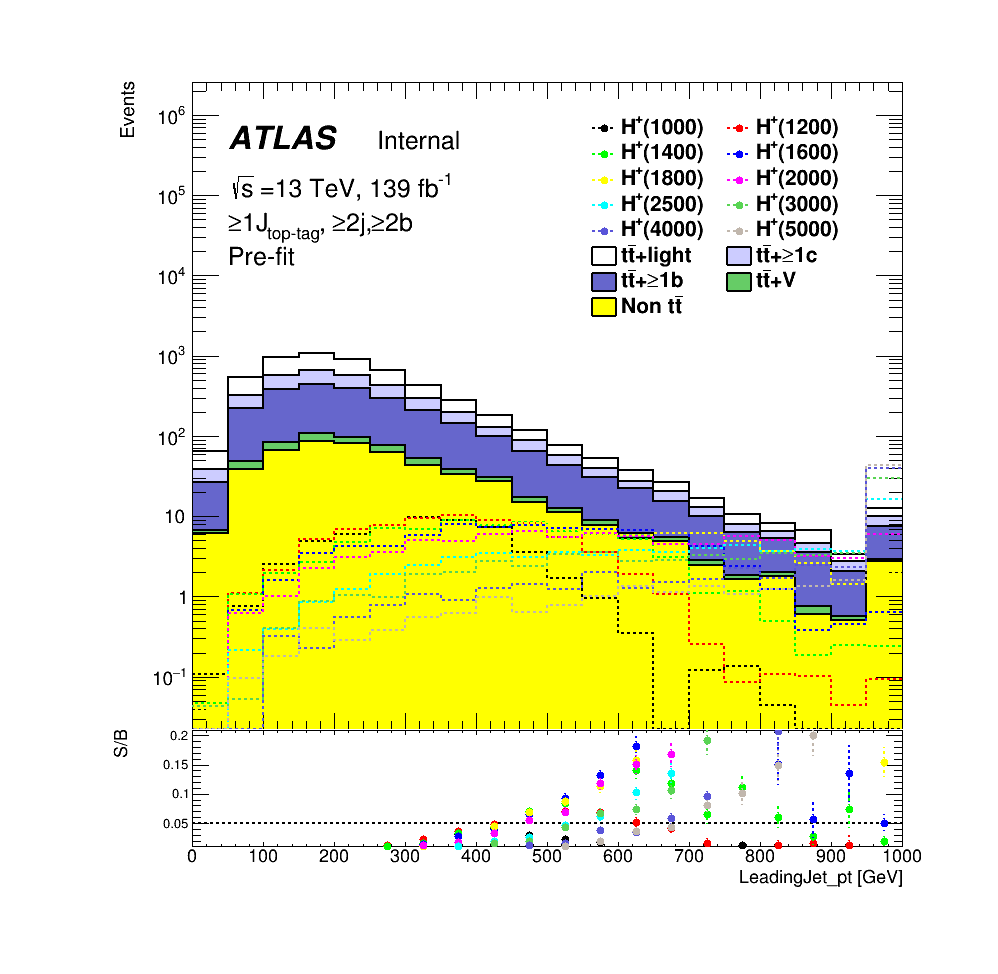
\includegraphics[width=0.50\textwidth]{images/SigBkgComparison/SOVERB_LeadingJet_pt_beforeRW_geq1tgeq2jgeq2b.png}
        \label{fig:SOVERB_LeadingJet_pt}
    }
\end{figure}
\begin{figure}[H]
    \addtocounter{figure}{-1}
    \subfloat[Centrality\_all] {
        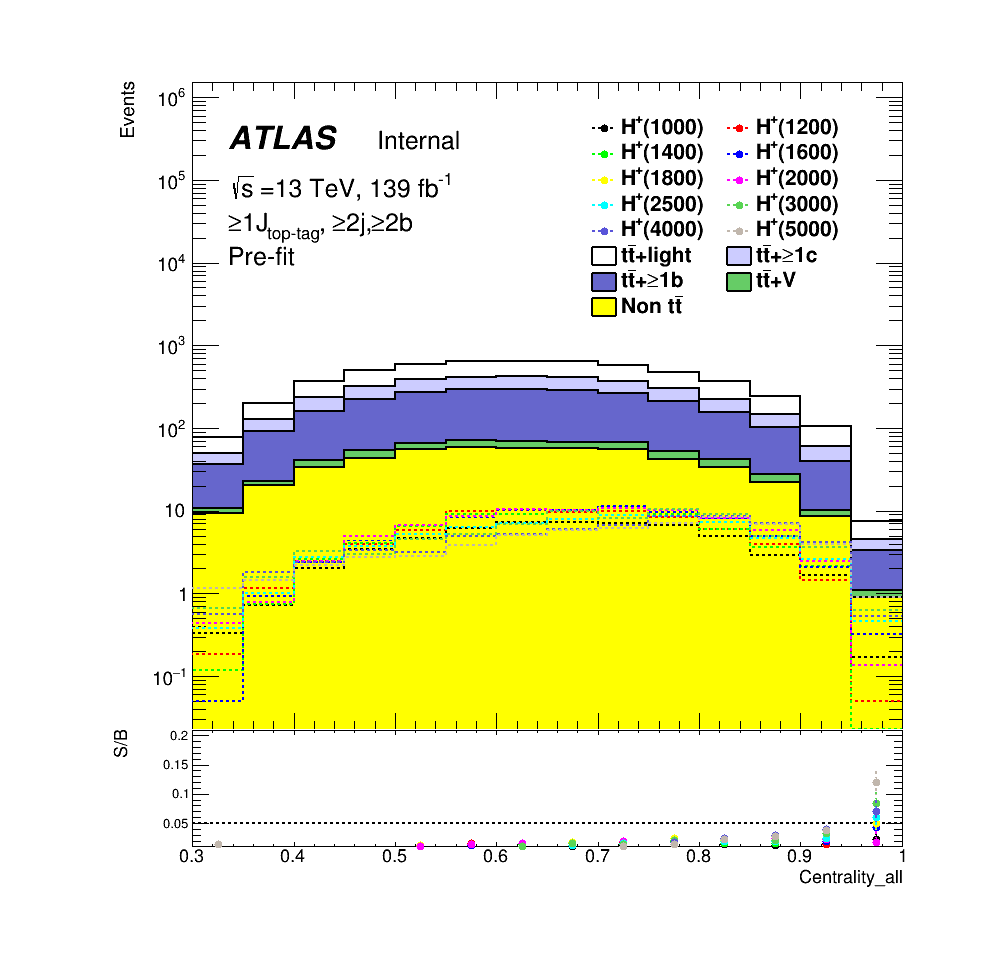
\includegraphics[width=0.50\textwidth]{images/SigBkgComparison/SOVERB_Centrality_all_beforeRW_geq1tgeq2jgeq2b.png}
        \label{fig:SOVERB_Centrality_all}
    }
    \subfloat[H1\_all] {
        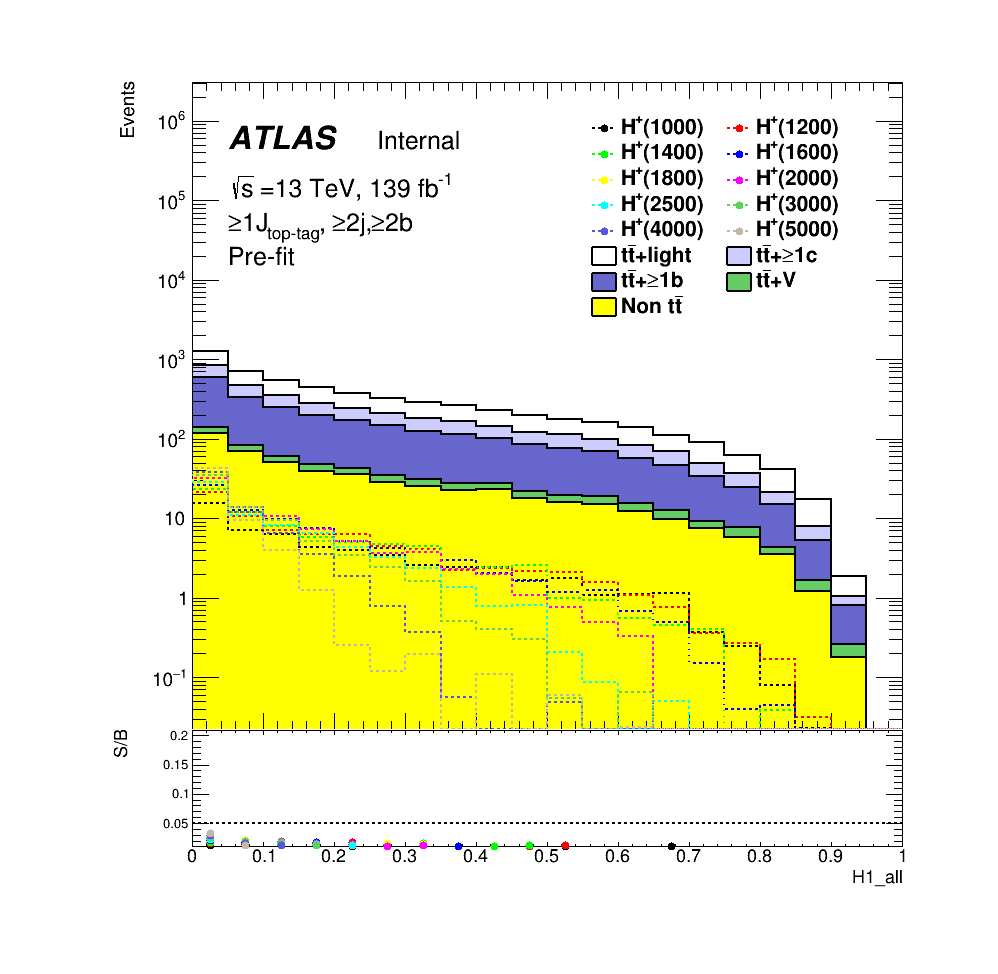
\includegraphics[width=0.50\textwidth]{images/SigBkgComparison/SOVERB_H1_all_beforeRW_geq1tgeq2jgeq2b.png}
        \label{fig:SOVERB_H1_all}
    }
\end{figure}
\begin{figure}[H]
    \subfloat[Mbb\_MaxPt] {
        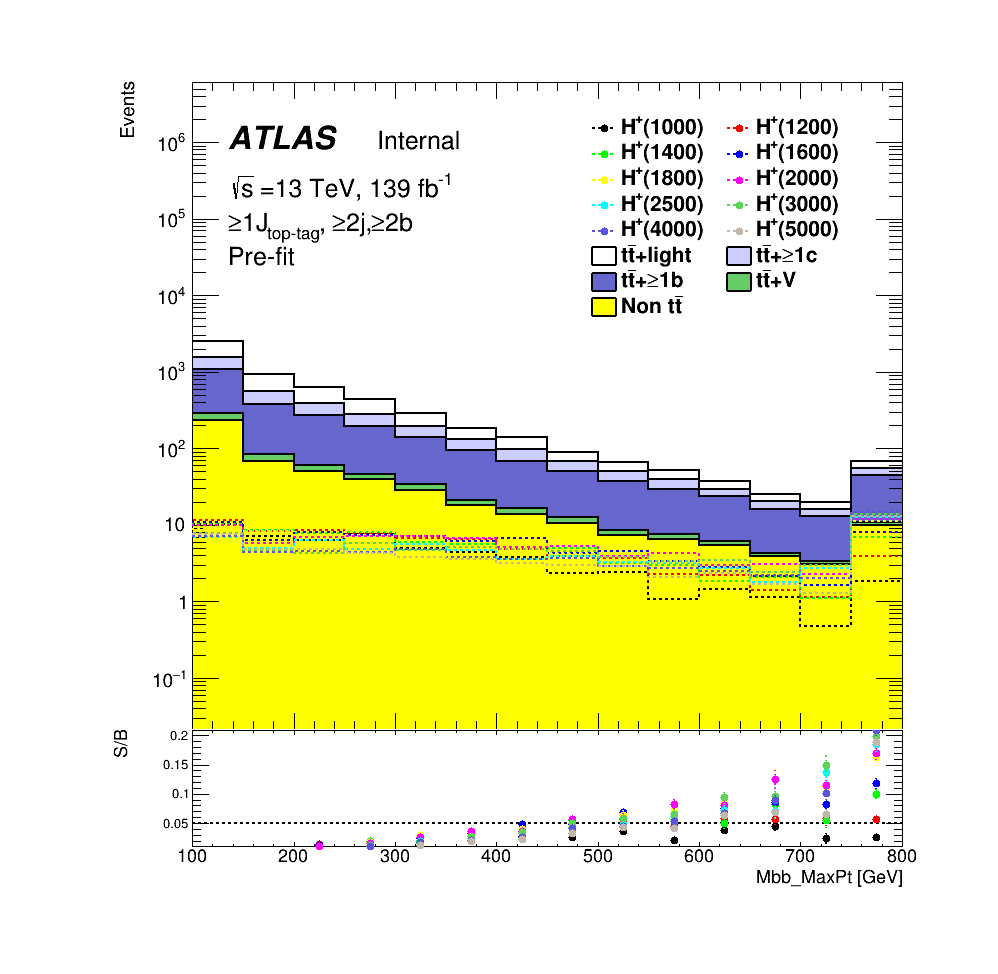
\includegraphics[width=0.50\textwidth]{images/SigBkgComparison/SOVERB_Mbb_MaxPt_beforeRW_geq1tgeq2jgeq2b.png}
        \label{fig:SOVERB_Mbb_MaxPt}
    }
    \subfloat[Mjjj\_MaxPt] {
        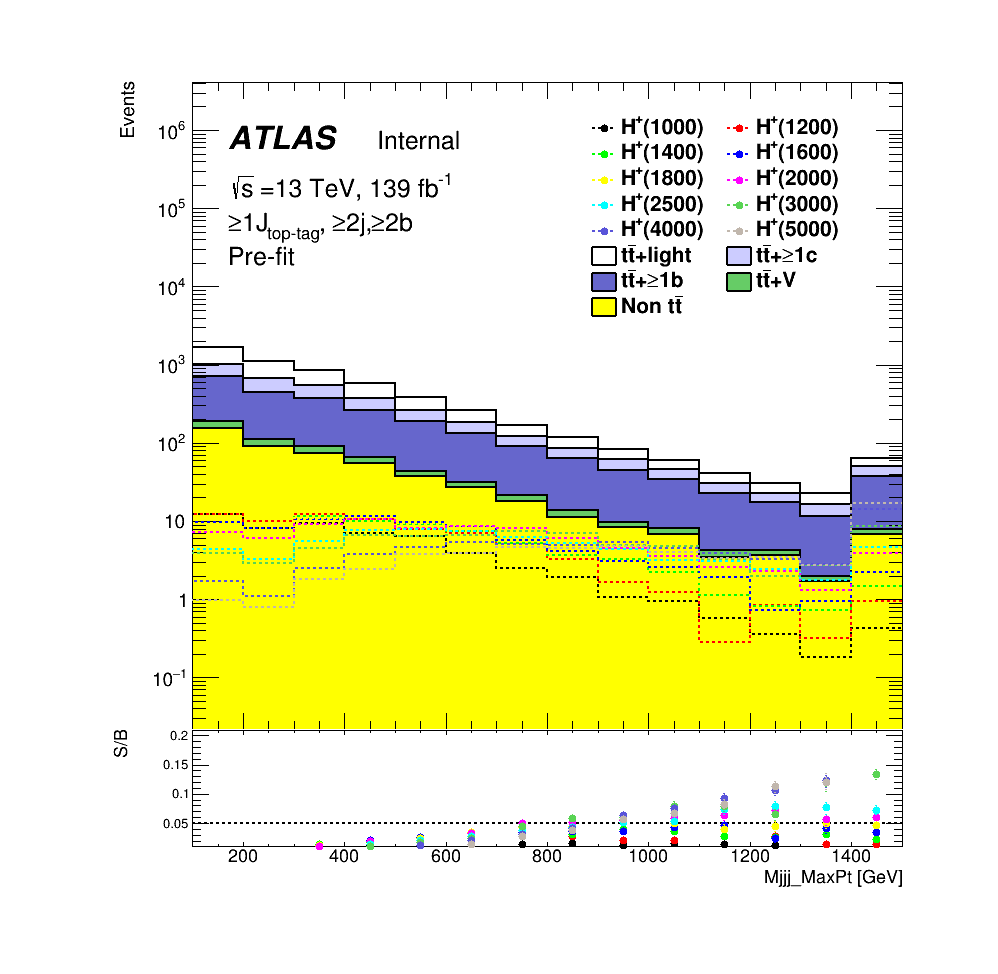
\includegraphics[width=0.50\textwidth]{images/SigBkgComparison/SOVERB_Mjjj_MaxPt_beforeRW_geq1tgeq2jgeq2b.png}
        \label{fig:SOVERB_Mjjj_MaxPt}
    }
\end{figure}
\begin{figure}[H]
    \subfloat[Muu\_MindR] {
        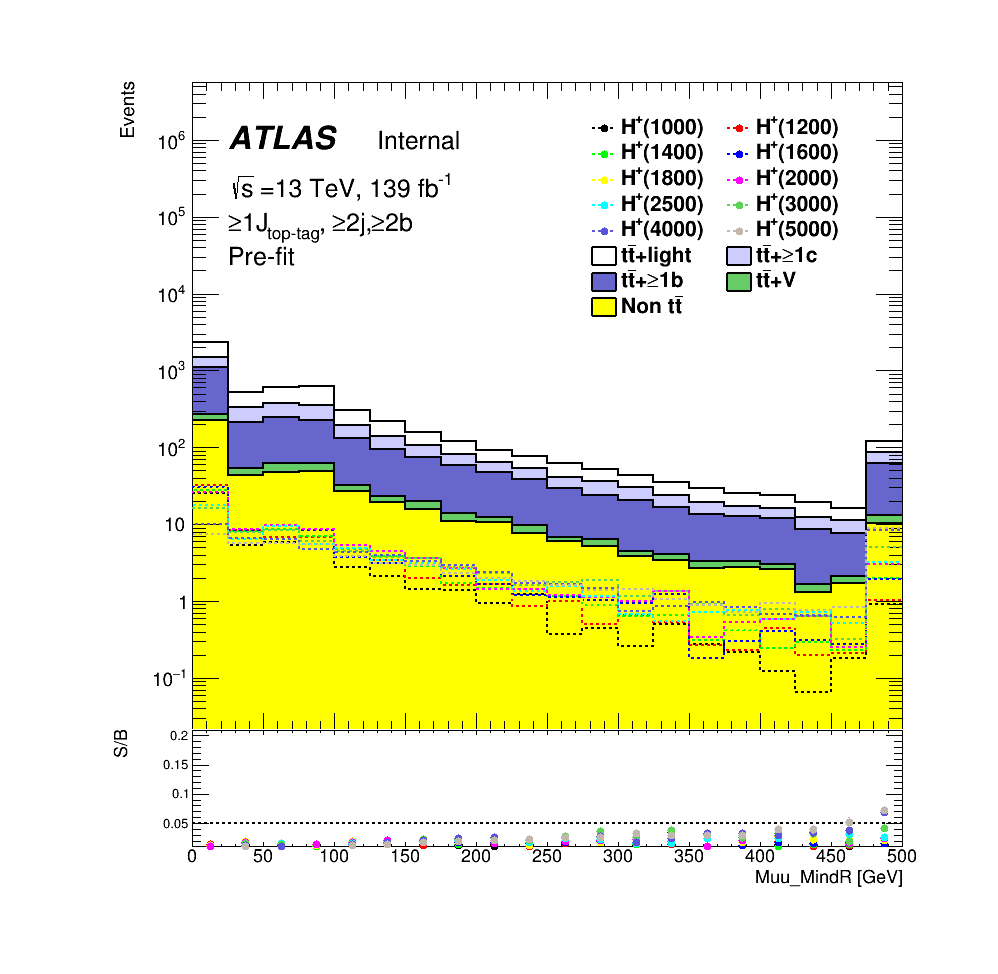
\includegraphics[width=0.50\textwidth]{images/SigBkgComparison/SOVERB_Muu_MindR_beforeRW_geq1tgeq2jgeq2b.png}
        \label{fig:SOVERB_Muu_MindR}
    }
    \subfloat[dRbb\_avg] {
        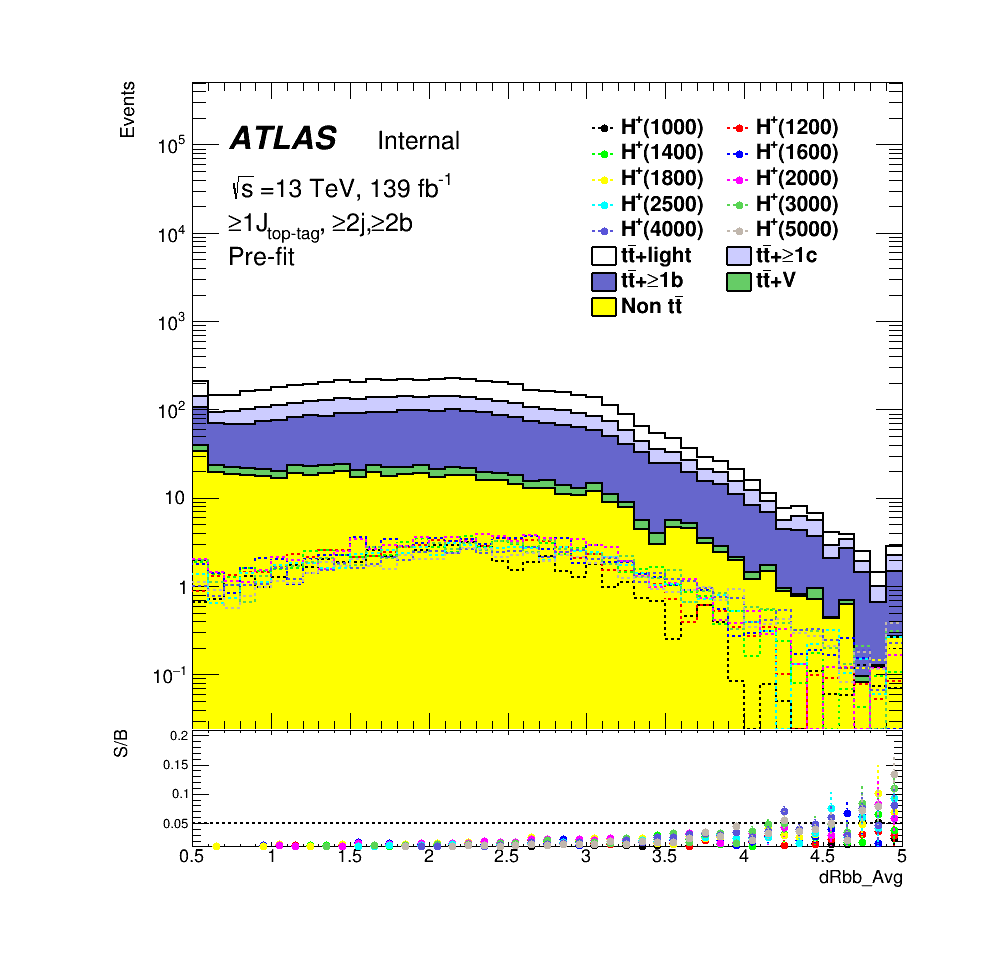
\includegraphics[width=0.50\textwidth]{images/SigBkgComparison/SOVERB_dRbb_avg_beforeRW_geq1tgeq2jgeq2b.png}
        \label{fig:SOVERB_dRbb_avg}
    }
\end{figure}
\begin{figure}[H]
    \subfloat[dRlepbb\_MindR] {
        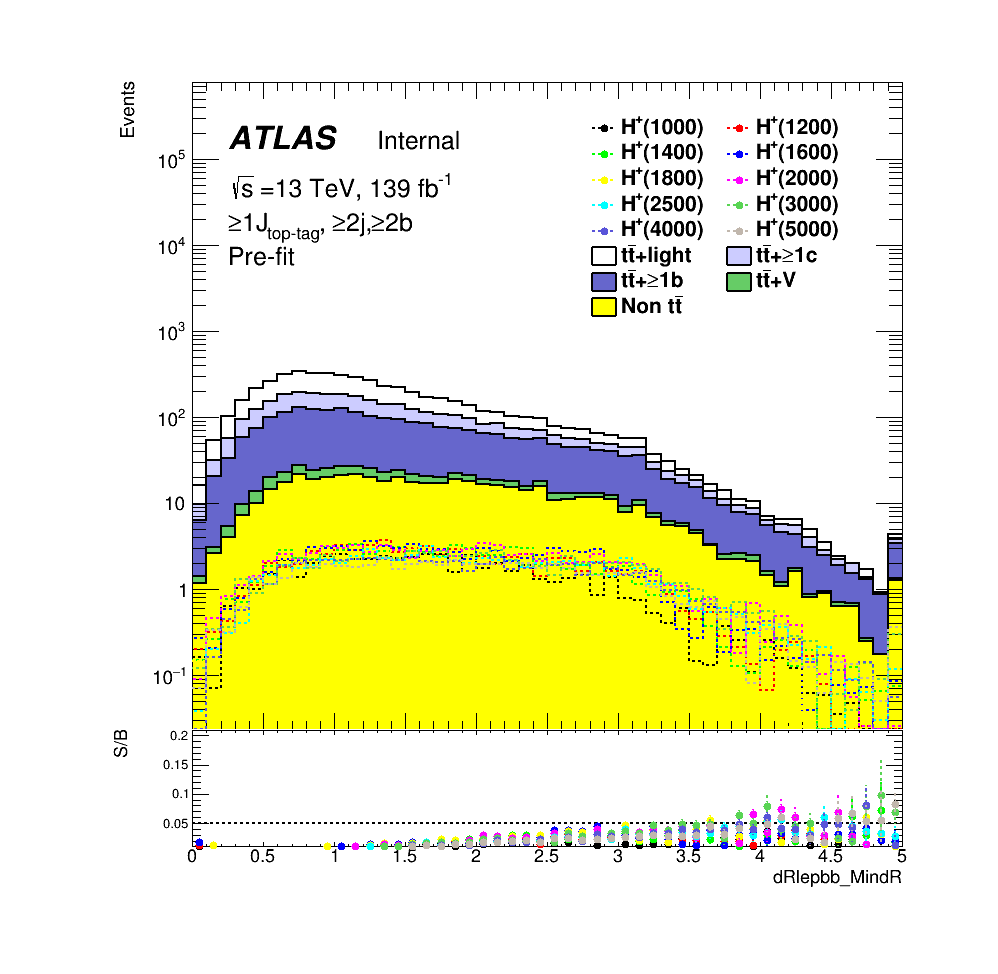
\includegraphics[width=0.50\textwidth]{images/SigBkgComparison/SOVERB_dRlepbb_MindR_beforeRW_geq1tgeq2jgeq2b.png}
        \label{fig:SOVERB_dRlepbb_MindR}
    }
    \subfloat[LeadingTop\_m] {
        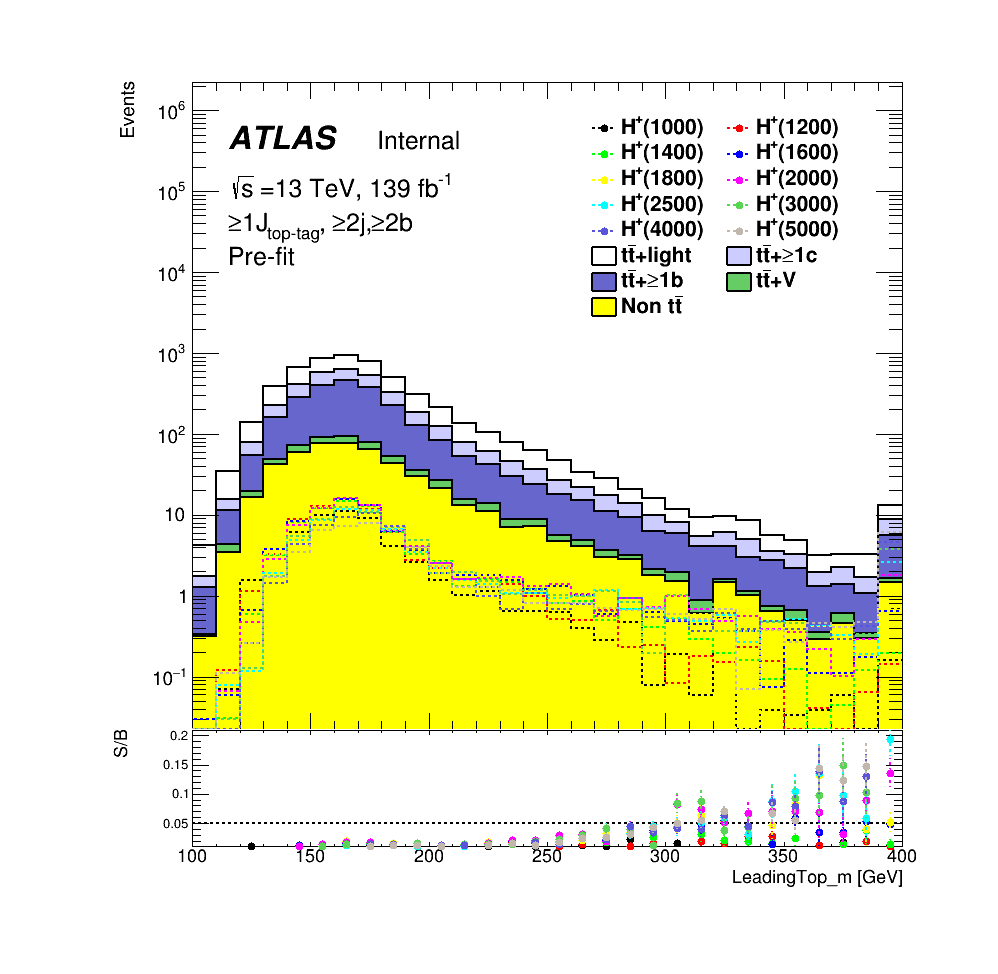
\includegraphics[width=0.50\textwidth]{images/SigBkgComparison/SOVERB_LeadingTop_mass_beforeRW_geq1tgeq2jgeq2b.png}
        \label{fig:SOVERB_LeadingTop_mass}
    }
\end{figure}
\begin{figure}[H]
    \subfloat[LeadingTop\_pt] {
        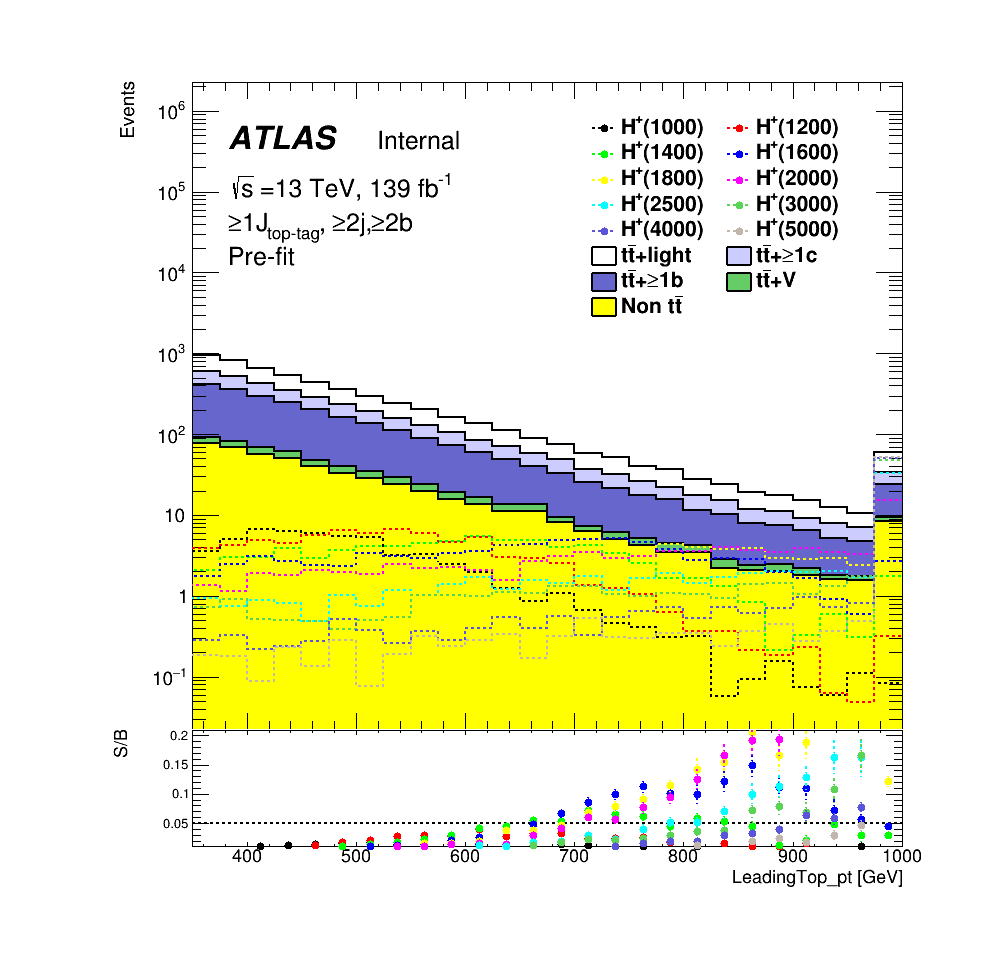
\includegraphics[width=0.50\textwidth]{images/SigBkgComparison/SOVERB_LeadingTop_pt_beforeRW_geq1tgeq2jgeq2b.png}
        \label{fig:SOVERB_LeadingTop_pt}
    }
    \subfloat[M\_tb] {
        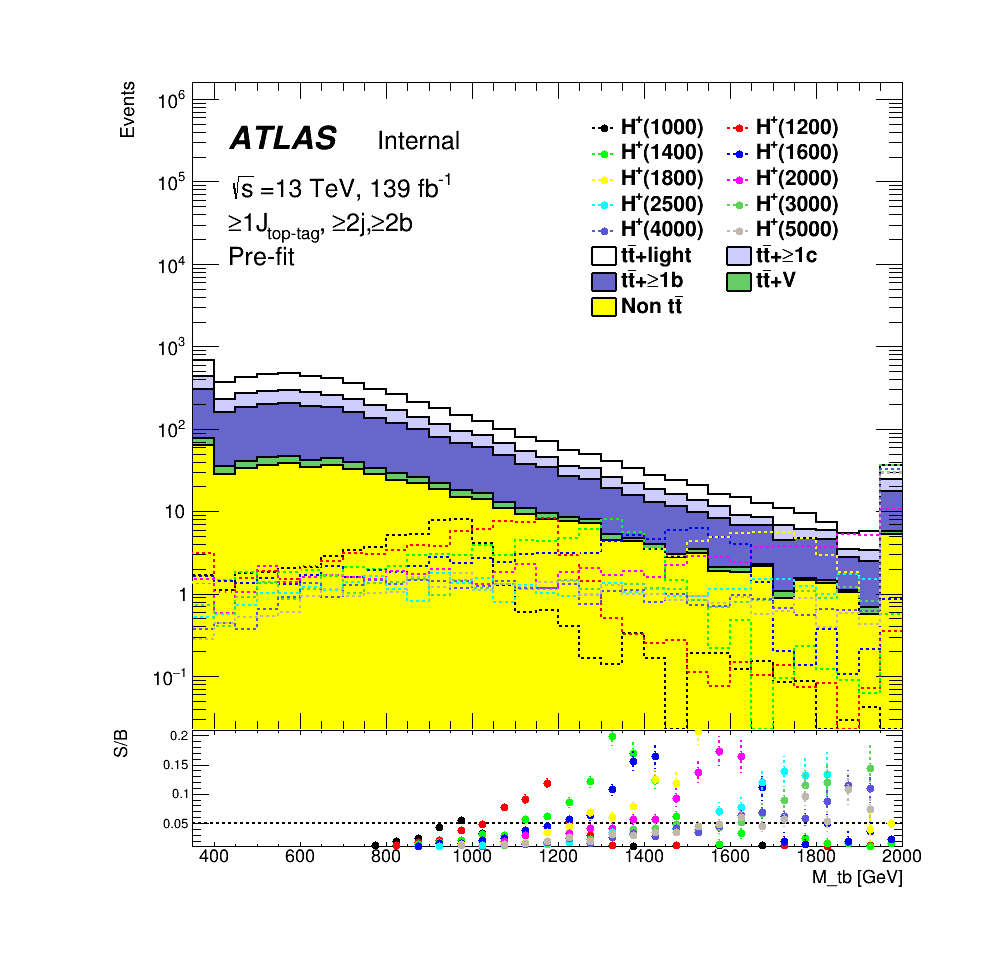
\includegraphics[width=0.50\textwidth]{images/SigBkgComparison/SOVERB_tb_mass_beforeRW_geq1tgeq2jgeq2b.png}
        \label{fig:SOVERB_tb_mass}
    }
\end{figure}
\begin{figure}[H]
    \subfloat[Pt\_tb] {
        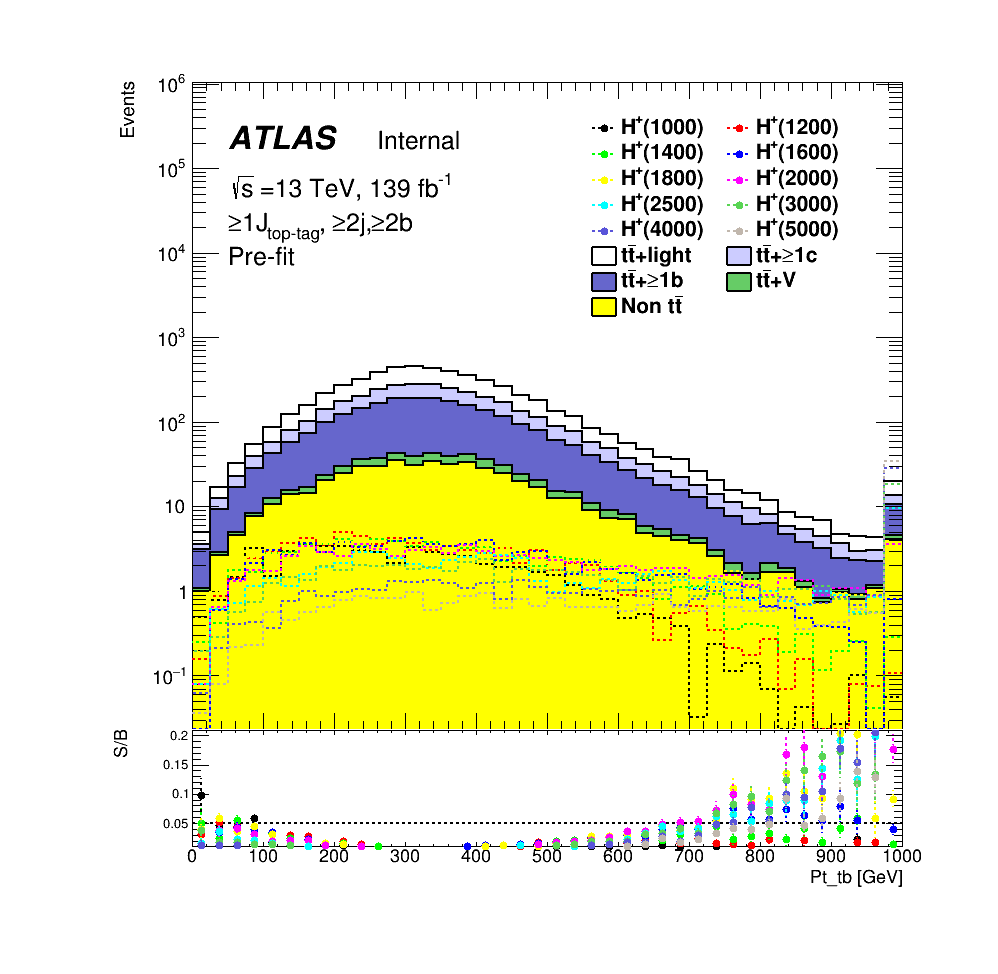
\includegraphics[width=0.50\textwidth]{images/SigBkgComparison/SOVERB_tb_pt_beforeRW_geq1tgeq2jgeq2b.png}
        \label{fig:SOVERB_tb_pt}
    }
    \subfloat[PtAsymm\_tb] {
        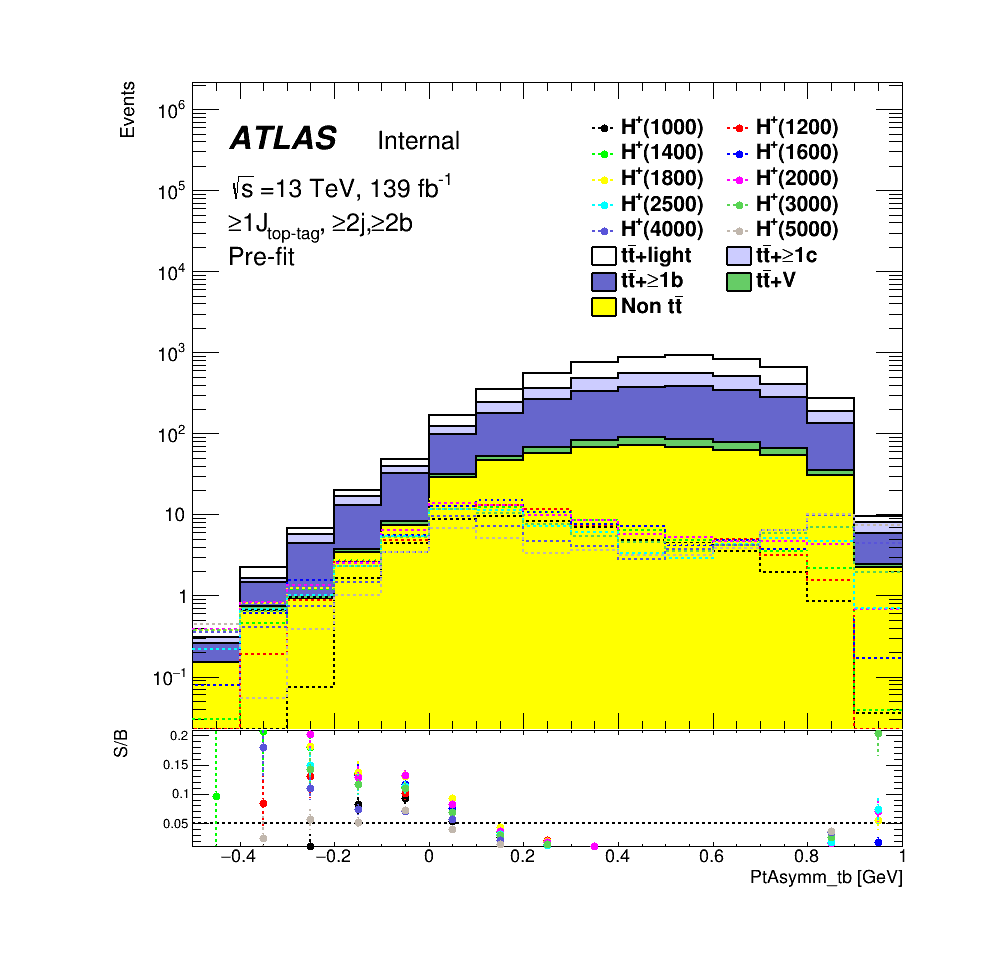
\includegraphics[width=0.50\textwidth]{images/SigBkgComparison/SOVERB_tb_ptAsymm_beforeRW_geq1tgeq2jgeq2b.png}
        \label{fig:SOVERB_tb_ptAsymm}
    }
    \caption{Comparison of the kinematic variables included in the BDT in the SR for the various $H^{+}$ signal masses between signal and background.}
    \label{fig:SOVERB_BDTInputs_Hp}
\end{figure}


\subsection{BDT outputs}
\label{subapp:SOVERB_BDTOutput}
Figures \ref{fig:SOVERB_BDT1000_Hp} to \ref{fig:SOVERB_BDT3000_Hp} compare the shape of BDT outputs for all $H^{+}$ signal masses and background in the SR.

\begin{figure}[H]
    \subfloat[BDT output@$H^{+}(1000)$] {
        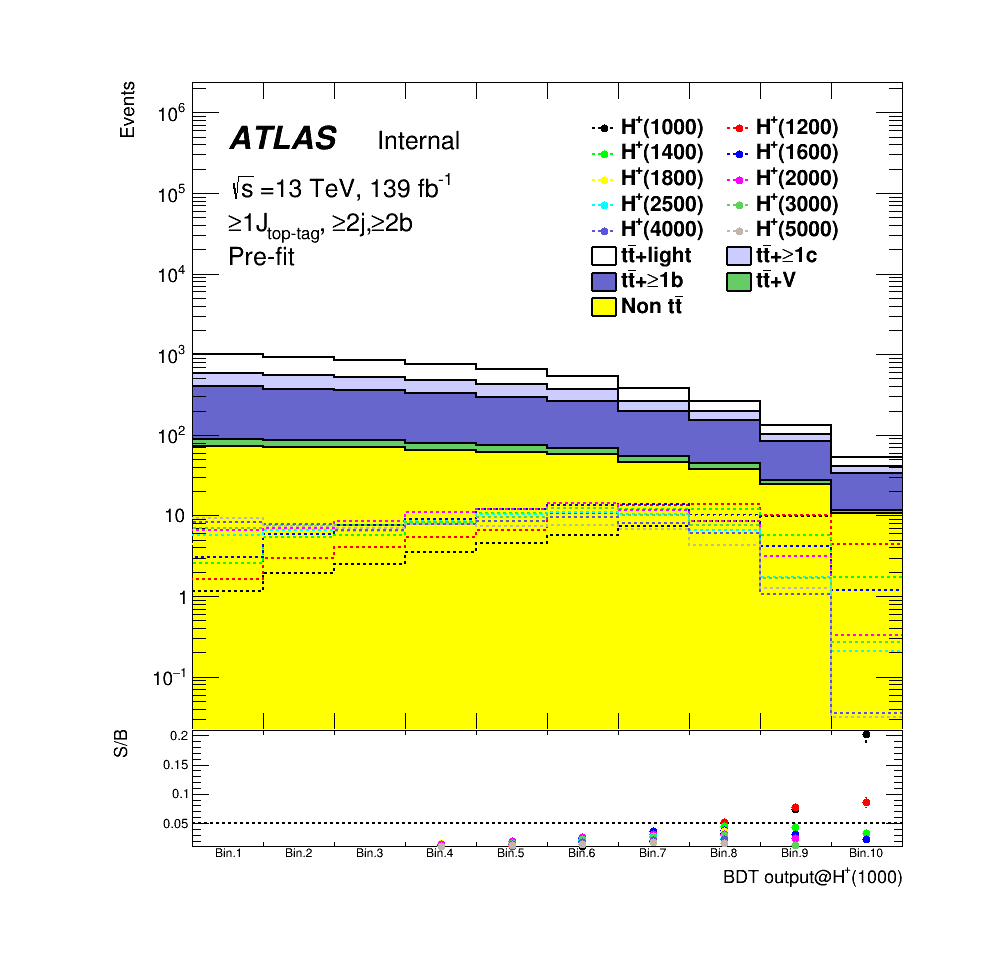
\includegraphics[width=0.50\textwidth]{images/SigBkgComparison/SOVERB_bdt_Hp1000_beforeRW_geq1tgeq2jgeq2b.png}
        \label{fig:SOVERB_BDT1000_Hp}
    }
    \subfloat[BDT output@$H^{+}(1200)$] {
        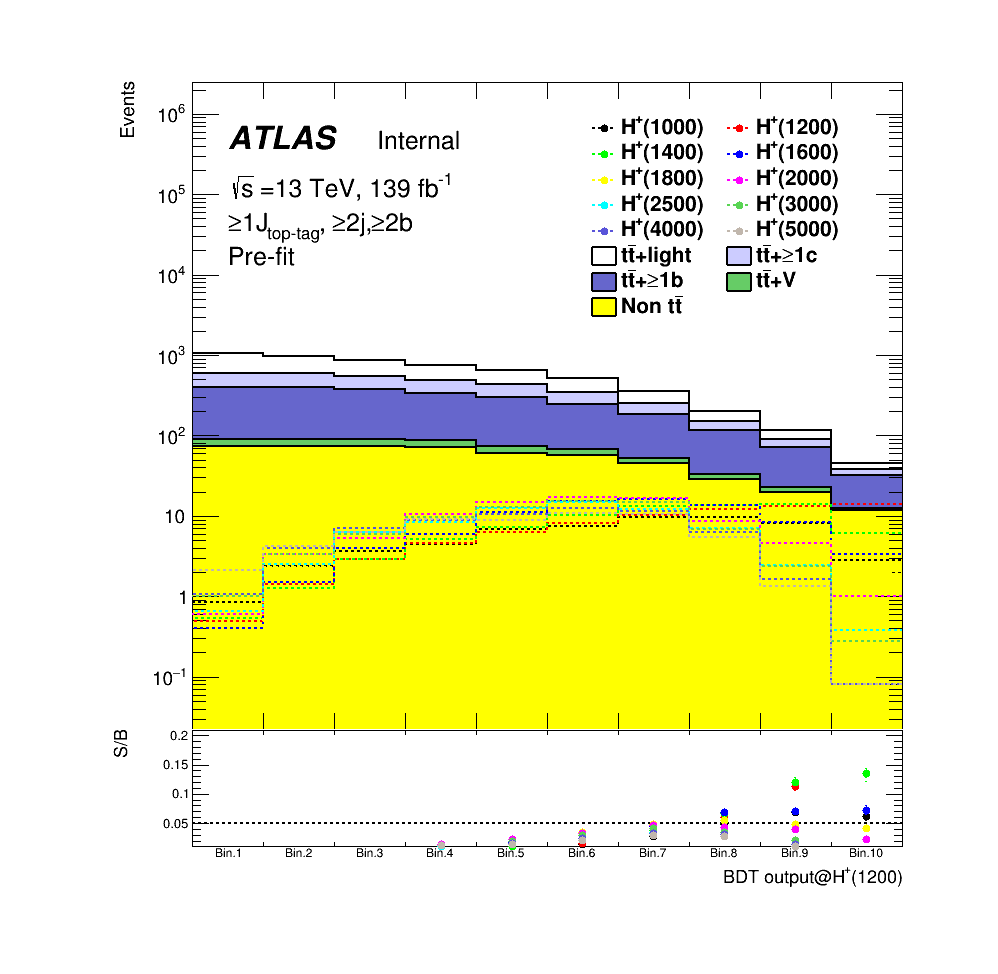
\includegraphics[width=0.50\textwidth]{images/SigBkgComparison/SOVERB_bdt_Hp1200_beforeRW_geq1tgeq2jgeq2b.png}
        \label{fig:SOVERB_BDT1200_Hp}
    }
\end{figure}
\begin{figure}[H]
    \subfloat[BDT output@$H^{+}(1400)$] {
        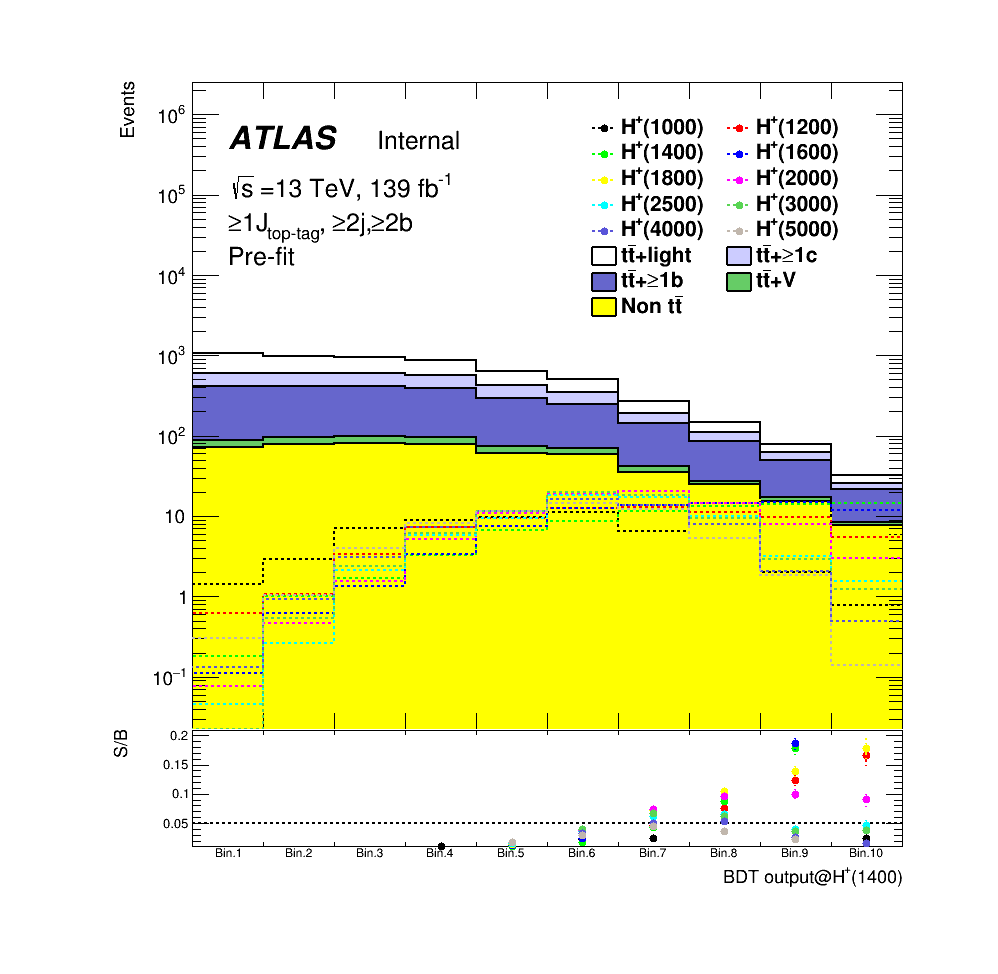
\includegraphics[width=0.50\textwidth]{images/SigBkgComparison/SOVERB_bdt_Hp1400_beforeRW_geq1tgeq2jgeq2b.png}
        \label{fig:SOVERB_BDT1400_Hp}
    }
    \subfloat[BDT output@$H^{+}(1600)$] {
        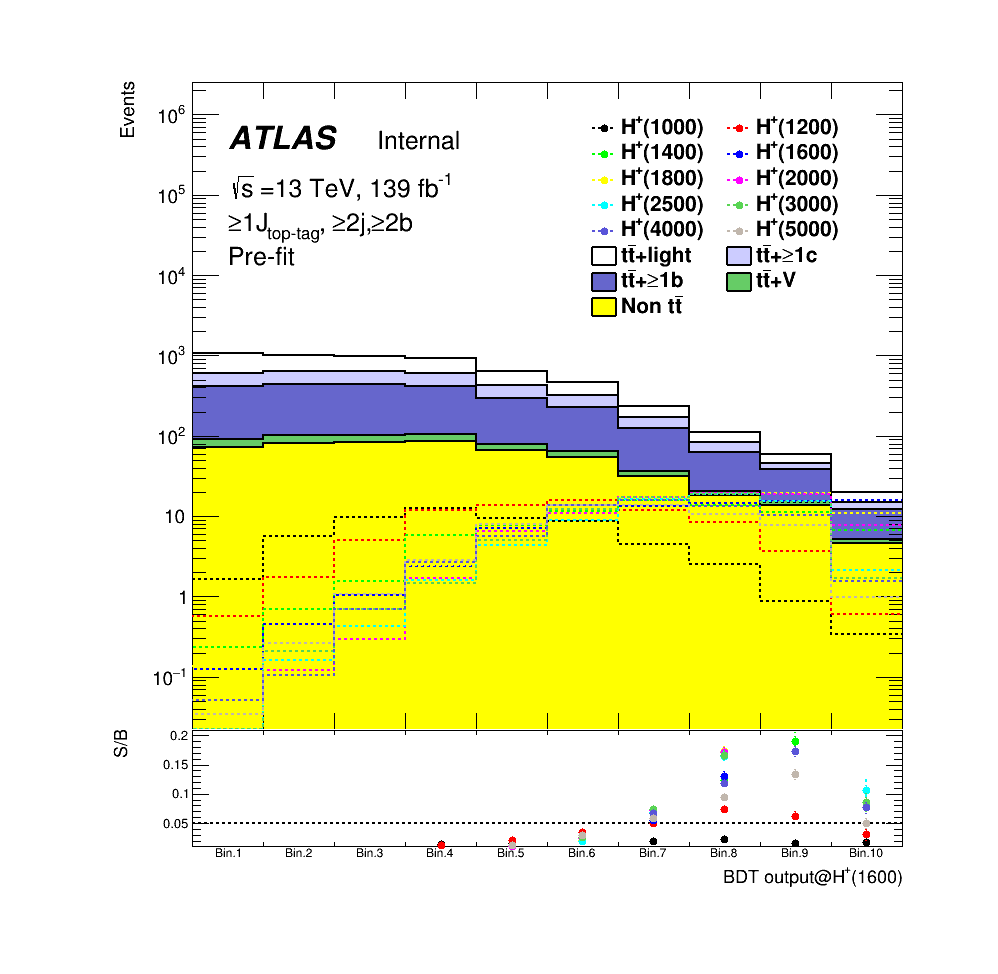
\includegraphics[width=0.50\textwidth]{images/SigBkgComparison/SOVERB_bdt_Hp1600_beforeRW_geq1tgeq2jgeq2b.png}
        \label{fig:SOVERB_BDT1600_Hp}
    }
\end{figure}
\begin{figure}[H]
    \subfloat[BDT output@$H^{+}(1800)$] {
        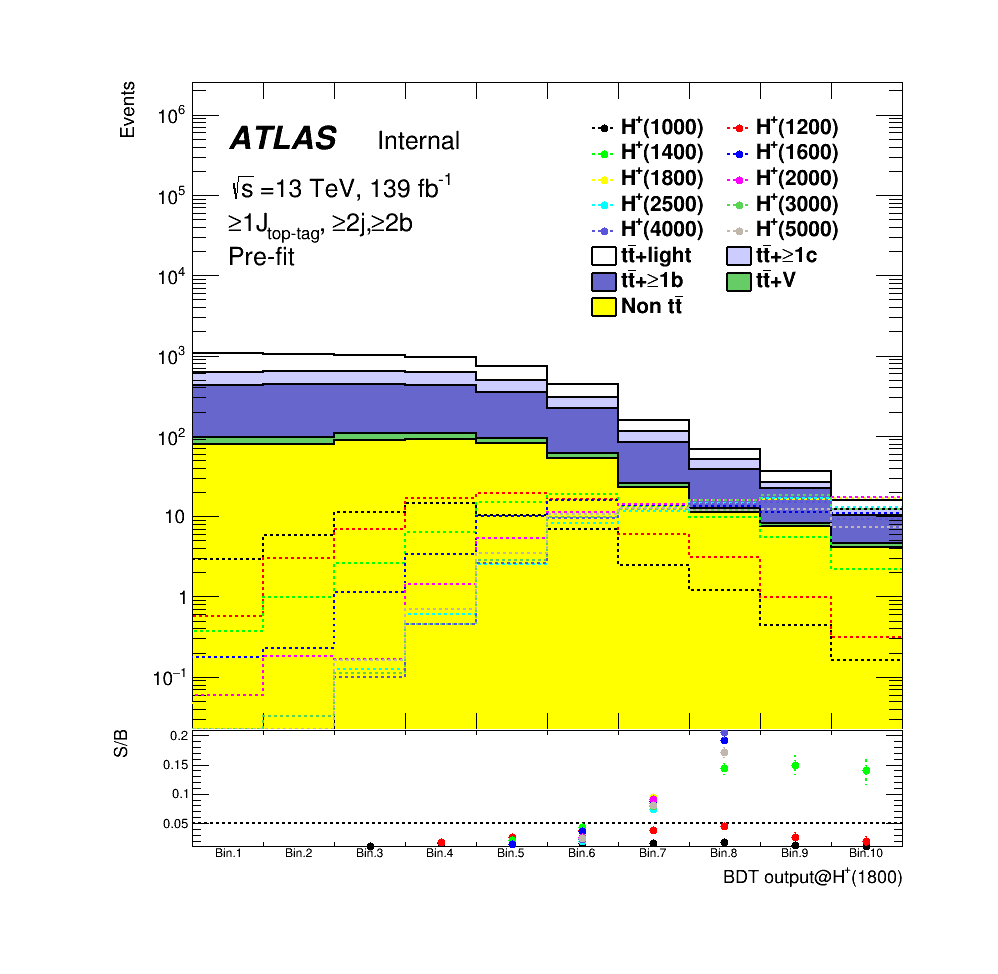
\includegraphics[width=0.50\textwidth]{images/SigBkgComparison/SOVERB_bdt_Hp1800_beforeRW_geq1tgeq2jgeq2b.png}
        \label{fig:SOVERB_BDT1800_Hp}
    }
    \subfloat[BDT output@$H^{+}(2000)$] {
        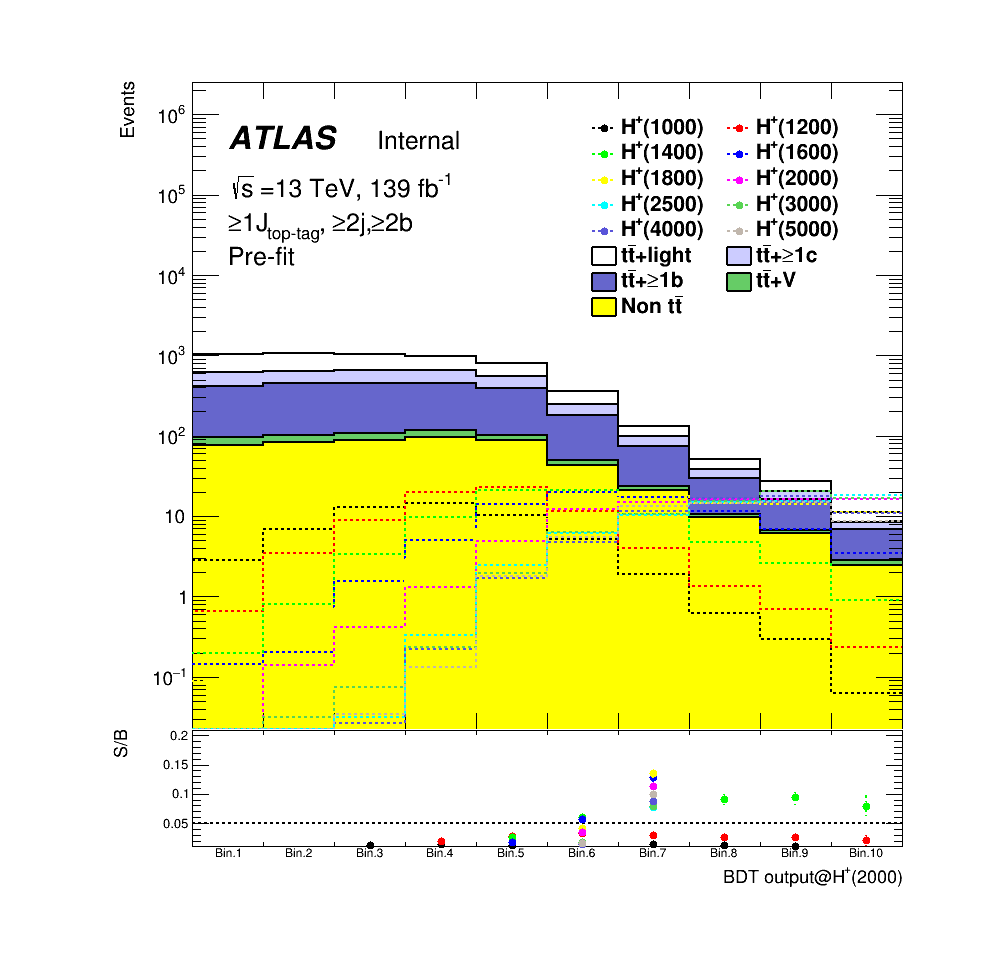
\includegraphics[width=0.50\textwidth]{images/SigBkgComparison/SOVERB_bdt_Hp2000_beforeRW_geq1tgeq2jgeq2b.png}
        \label{fig:SOVERB_BDT2000_Hp}
    }
\end{figure}
\begin{figure}[H]
    \subfloat[BDT output@$H^{+}(2500)$] {
        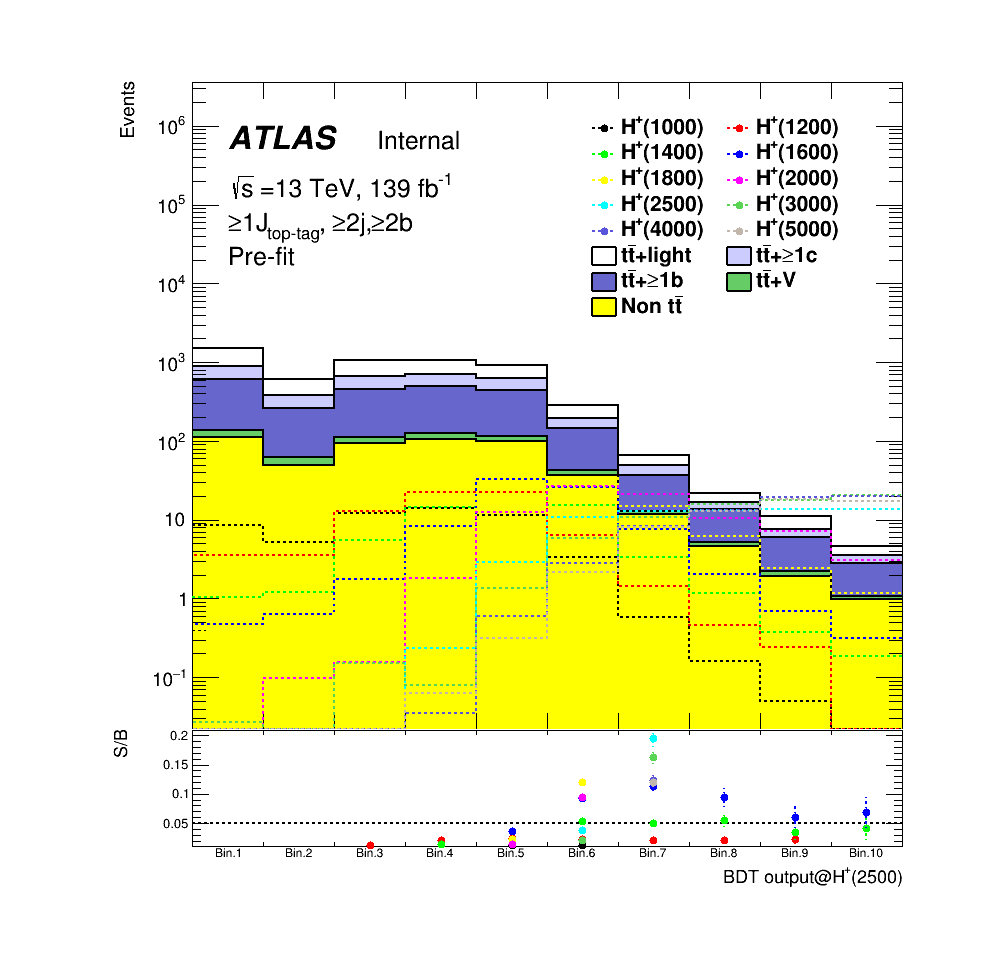
\includegraphics[width=0.50\textwidth]{images/SigBkgComparison/SOVERB_bdt_Hp2500_beforeRW_geq1tgeq2jgeq2b.png}
        \label{fig:SOVERB_BDT2500_Hp}
    }
    \subfloat[BDT output@$H^{+}(3000)$] {
        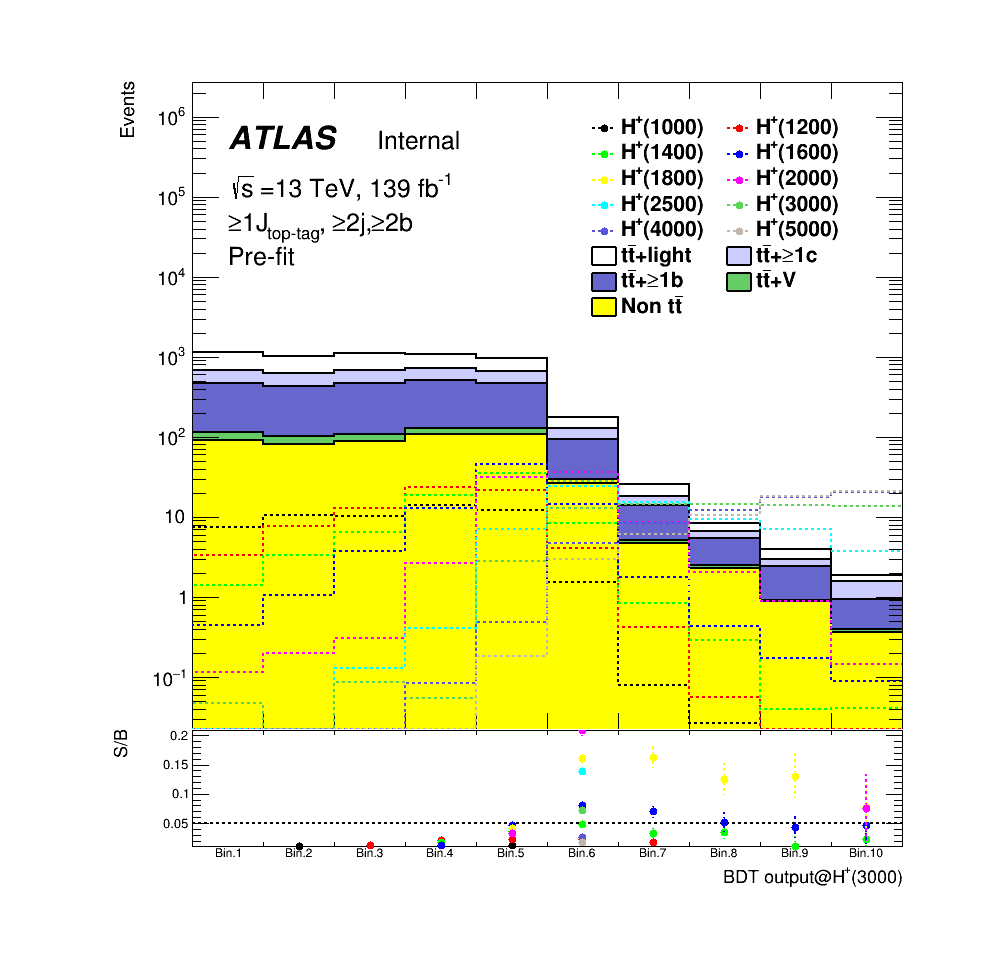
\includegraphics[width=0.50\textwidth]{images/SigBkgComparison/SOVERB_bdt_Hp3000_beforeRW_geq1tgeq2jgeq2b.png}
        \label{fig:SOVERB_BDT3000_Hp}
    }
    \caption{Comparison of BDT outputs in the SR for the various $H^{+}$ signal masses between signal and background.}
    \label{fig:SOVERB_BDTOutputs_Hp}
\end{figure}


\subsection{$H_{\text{T}}^{\text{jets}}$ in the CR}
\label{subapp:SOVERB_HTjets_1b}
Figure \ref{fig:SOVERB_BDTInputs_Hp} compares the shape of $H_{\text{T}}^{\text{jets}}$ for all $H^{+}$ signal masses and background in the CR.

\begin{figure}[H]
    \centering
    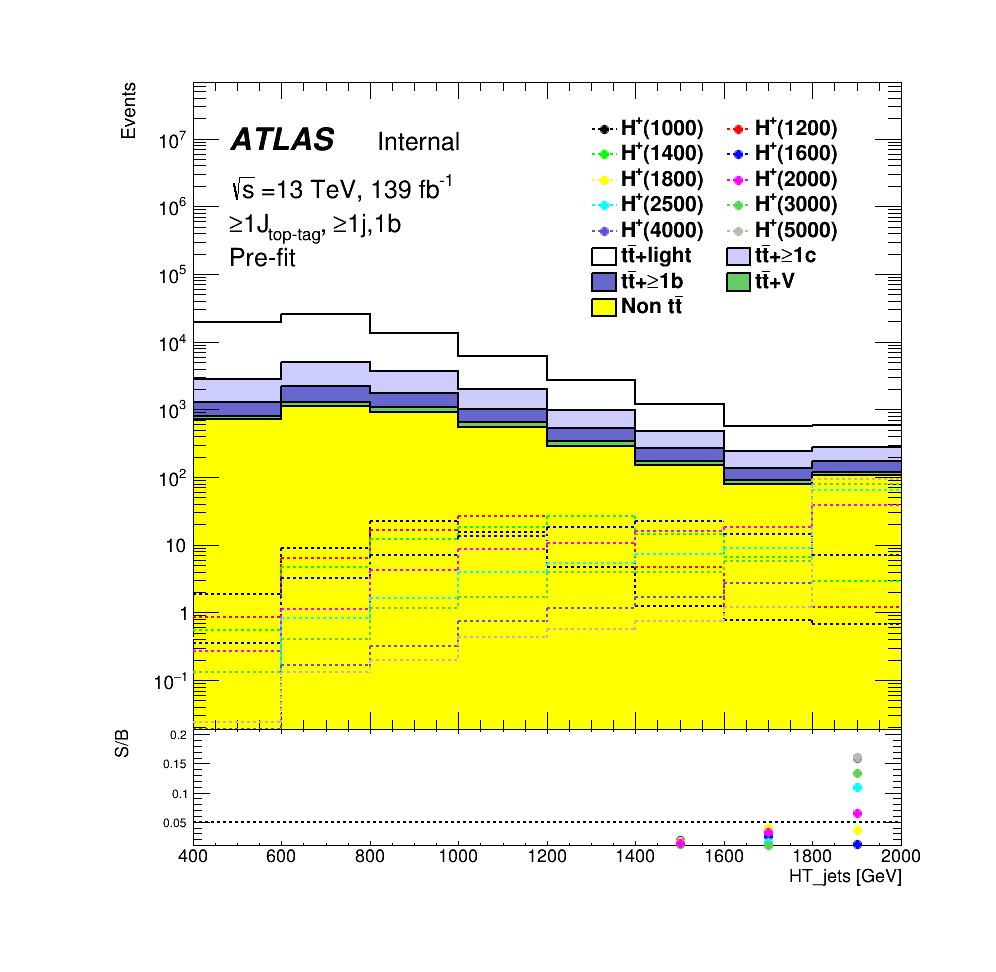
\includegraphics[width=0.50\textwidth]{images/SigBkgComparison/SOVERB_HTjets_beforeRW_geq1tgeq1j1b.png}
    \caption{Comparison of $H_{\text{T}}^{\text{jets}}$ in the CR for the various $H^{+}$ signal masses between signal and background.}
    \label{fig:SOVERB_BDTInputs_Hp}
\end{figure}